%\section{Features at a Glance}\label{feature_glance}

\section{Aperçu des fonctionnalités}\label{feature_glance}

% when the revision of a section has been finalized, 
% comment out the following line:
%\updatedisclaimer

%After a first and simple sample session in Section \ref{label_getstarted} we now 
%want to give you a more detailed overview of the features of QGIS. 
%Most features presented in the following chapters will be explained and described in 
%own sections later in the manual.

Après une première prise en main dans le chapitre \ref{label_getstarted}, nous allons maintenant vous donner un aperçu plus détaillé des fonctionnalités de QGIS. La plupart seront décrites plus précisément dans les chapitres qui leur sont dédiés dans la suite du manuel.

%\subsection{Starting and Stopping QGIS}\label{label_startinqgis}
%
%In Section \ref{samplesession} you already learned how to start QGIS. We will 
%repeat this here and you will see that QGIS also provides further command line options. 

\subsection{Démarrer et arrêter QGIS}\label{label_startinqgis}

Dans le chapitre \ref{samplesession} vous avez appris comment démarrer QGIS ? Nous allons le répéter ici et vous verrez que QGIS propose des options supplémentaires via la ligne de commande.

%\begin{itemize}
%\item \nix{assuming that QGIS is installed in the PATH, you can start QGIS 
%by typing: \usertext{qgis}  at a command prompt or by double clicking on the QGIS
%application link (or shortcut) on the desktop.} 
%\item \win{start QGIS using the Start menu or desktop shortcut, 
%or double click on a QGIS project file.}
%\item \osx{double click the icon in your Applications folder.}
%\end{itemize} 

\begin{itemize}
\item \nix{en présumant que QGIS est installé dans le PATH (chemin par défaut), vous pouvez le démarrez en tapant : \usertext{qgis}  dans une ligne de commande ou en cliquant sur l'icône de raccourci.} 
\item \win{démarrez QGIS en utilisant le menu Démarrer, l'icône de raccourci présent sur le bureau ou encore, en cliquant sur un fichier de projet QGIS}
\item \osx{double-cliquez sur l'icône de votre répertoire Applications.}
\end{itemize} 

%To stop QGIS, click the menu options \{\nix{}\win{File} \osx{QGIS}\} > Quit,
%or use the shortcut \keystroke{Ctrl+Q}.

Pour arrêter QGIS, cliquez sur le menu \{\nix{}\win{Fichier} \osx{QGIS}\} > Quitter, ou utilisez le raccourci clavier \keystroke{Ctrl+Q}.

%\subsubsection{Command Line Options}\index{command line options}
%\label{label_commandline}

\subsubsection{Options de ligne de commande}\index{command line options}
\label{label_commandline}

%\nix QGIS supports a number of options when started from the command line. To
%get a list of the options, enter \usertext{qgis ---help} on the command line.
%The usage statement for QGIS is:

\nix QGIS supporte un certain nombre d'options lorsque démarrer en passant par la ligne de commande. Pour obtenir une liste de ces options, entrez dans votre console \usertext{qgis ---help}. Le message habituel qui en résulte est :

%\small
%\begin{verbatim}
%qgis --help
%Quantum GIS - 1.0.0 'Kore'
%Quantum GIS (QGIS) is a viewer for spatial data sets, including
%raster and vector data.
%Usage: qgis [options] [FILES]
%  options:
%        [--snapshot filename]   emit snapshot of loaded datasets to given file
%        [--lang language]       use language for interface text
%        [--project projectfile] load the given QGIS project
%        [--extent xmin,ymin,xmax,ymax]  set initial map extent
%        [--help]                this text
%
%  FILES:
%    Files specified on the command line can include rasters,
%    vectors, and QGIS project files (.qgs):
%     1. Rasters - Supported formats include GeoTiff, DEM
%        and others supported by GDAL
%     2. Vectors - Supported formats include ESRI Shapefiles
%        and others supported by OGR and PostgreSQL layers using
%        the PostGIS extension
%\end{verbatim}
%\normalsize

\small
\begin{verbatim}
qgis --help
Quantum GIS - 1.0.0 'Kore'
Quantum GIS (QGIS) est un visualisateur de données spatiales, raster ou vecteur.
Usage: qgis [options] [FILES]
  options:
        [--snapshot filename]   emit snapshot of loaded datasets to given file
        [--lang language]       use language for interface text
        [--project projectfile] load the given QGIS project
        [--extent xmin,ymin,xmax,ymax]  set initial map extent
        [--help]                this text

  FILES:
    Files specified on the command line can include rasters,
    vectors, and QGIS project files (.qgs):
     1. Rasters - Supported formats include GeoTiff, DEM
        and others supported by GDAL
     2. Vectors - Supported formats include ESRI Shapefiles
        and others supported by OGR and PostgreSQL layers using
        the PostGIS extension
\end{verbatim}
\normalsize

%\begin{Tip} \caption{\textsc{Example Using command line arguments}}
%\qgistip{You can start QGIS by specifying one or more data files
%on the command line. For example, assuming you are in the 
%qgis\_sample\_data directory, you could start QGIS with a vector layer 
%and a raster file set to load on startup using the following command: 
%\usertext{qgis ./raster/landcover.img ./gml/lakes.gml}
%}
%\end{Tip}

\begin{Astuce} \caption{\textsc{Exemple utilisant des options de ligne de commande}}
\qgistip{Vous pouvez démarrer QGIS en spécifiant un ou plusieurs fichiers de données. Par exemple, si vous êtes placé dans le répertoire qgis\_sample\_data vous pouvez démarrer QGIS avec une couche vecteur et un fichier raster dès le démarrage avec la commande suivante : 
\usertext{qgis ./raster/landcover.img ./gml/lakes.gml}
}
\end{Astuce}

%\minisec{Command line option \usertext{---snapshot}}
%This option allows you to create a snapshot in PNG format from the current view.
%This comes in handy when you have a lot of projects and want to 
%generate snapshots from your data.
%
%Currently it generates a PNG-file with 800x600 pixels. A filename can be added after
%\usertext{---snapshot}.

\minisec{Option \usertext{---snapshot}}
Cette option permet de créer une capture d'écran de l'affichage courant au format PNG. C'est pratique quand vous avez une longue série de projets et que vous voulez générer un aperçu de vos données. L'image ainsi créée fait 800x600 pixels, un nom de fichier peut être ajouté après \usertext{---snapshot}.

%\minisec{Command line option \usertext{---lang}}
%Based on your locale QGIS, selects the correct localization. If you would like 
%to change your language, you can specify a language code. For example: 
%\usertext{---lang=it}
%starts QGIS in italian localization. A list of currently supported
%languages with language code is provided at
%\url{http://wiki.qgis.org/qgiswiki/TranslatorsCorner} 

\minisec{Option \usertext{---lang}}
QGIS se base sur vos paramètres globaux pour définir la langue de l'interface. Si vous voulez en changer, vous devez le spécifier en saisissant un code. 
Par exemple, \usertext{---lang=it} provoquera l'utilisation de la version italienne. Une liste des langues intégrées est visible à \url{http://wiki.qgis.org/qgiswiki/TranslatorsCorner} 

%\minisec{Command line option \usertext{---project}}
%Starting QGIS with an existing project file is also possible. Just
%add the command line option \usertext{--project} followed by your project name
%and QGIS will open with all layers loaded described in the given file.

\minisec{COption \usertext{---project}}
Démarrer QGIS avec un projet existant est possible, il suffit de rajouter cette option suivie du nom de votre projet et QGIS se lancera avec toutes les couches de ce fichier.

%\minisec{Command line option \usertext{---extent}}
%To start with a specific map extent use this option. You need to add the bounding
%box of your extent in the following order separated by a comma:
%\begin{verbatim}
%--extent xmin,ymin,xmax,ymax
%\end{verbatim}

\minisec{Option \usertext{---extent}}
Pour démarrer avec une étendue cartographique spécifique, utilisez cette option. Vous devez ajouter les limites de votre étendue dans l'ordre suivant en les séparant par une virgule :
\begin{verbatim}
--extent xmin,ymin,xmax,ymax
\end{verbatim}

%\subsection{QGIS GUI}\index{main window}
%\label{label_qgismainwindow}

\subsection{Interface de QGIS}\index{fenêtre principale}
\label{label_qgismainwindow}

%When QGIS starts, you are presented with the GUI as shown below
%(the numbers 1 through 6 in yellow ovals refer to the six major areas of the
%interface as discussed below):
%
%\begin{figure}[ht]
%   \begin{center}
%   \caption{QGIS GUI with Alaska sample data \wincaption}
%  \label{fig:startup}
%   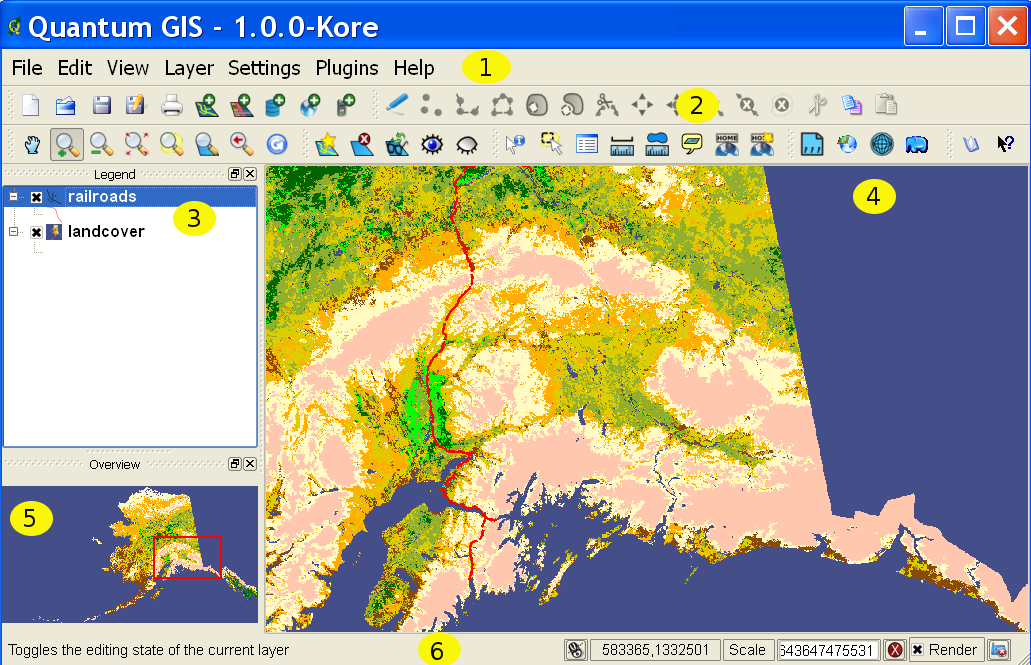
\includegraphics[clip=true, width=17cm]{startup1_0_0}
%\end{center} 
%\end{figure}
%
%\textbf{Note:} Your window decorations (title bar, etc.) may appear
%different depending on your operating system and window manager.

Quand QGIs démarre, l'interface se présente à vous sous la forme affichée ci-dessous (les nombres de 1 à 6 se réfèrent aux six zones majeures de l'interface) :

\begin{figure}[ht]
   \begin{center}
   \caption{Interface de QGIS avec les données d'essai de l'Alaska \nixcaption}
  \label{fig:startup}
   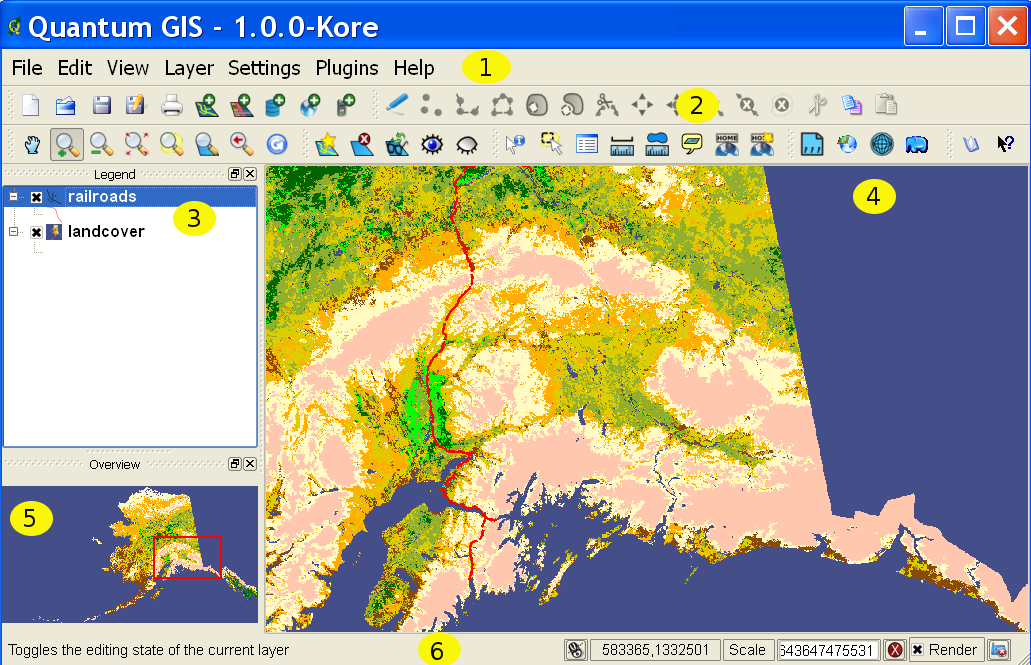
\includegraphics[clip=true, width=17cm]{startup1_0_0}
\end{center} 
\end{figure}

\textbf{Note:} Les décorations de fenêtre peuvent vous apparaître différemment sur votre système en fonction de votre système d'exploitation et de votre gestionnaire de fenêtre.

%The QGIS GUI is divided into six areas:
%
%\begin{tabbing}
%1. Menu Bar \hspace{3cm}\= 4. Map View \\
%2. Tool Bar \hspace{3cm}\> 5. Map Overview  \\
%3. Map Legend \hspace{3cm}\> 6. Status Bar   
%\end{tabbing}
%
%These six components of the QGIS interface are described in more detail in
%the following sections.

L'interface est divisée en 6 zones distinctes :

\begin{tabbing}
1. Barre de Menu \hspace{3cm}\= 4. Affichage de la carte \\
2. Barre d'Outils \hspace{3cm}\> 5. Aperçu de la carte  \\
3. Légende de la carte \hspace{3cm}\> 6. Barre de statut   
\end{tabbing}

Ces 6 composants sont décrits dans les sections suivantes.

%\subsubsection{Menu Bar}\label{label_menubar}
%\index{menus}
%
%The menu bar provides access to various QGIS features using a standard 
%hierarchical menu. The top-level menus and a summary of some of the
%menu options are listed below, together with the icons of the corresponding 
%tools as they appear on the toolbar, as well as keyboard shortcuts.
%Although most menu options have a corresponding tool and vice-versa,
%the menus are not organized quite like the toolbars. 
%The toolbar containing the tool is listed after each menu option as a checkbox
%entry. For more information about tools and toolbars, see Section \ref{label_toolbars}.

\subsubsection{Barre de Menu}\label{label_menubar}
\index{menus}

La barre de menu fournit un accès aux différentes fonctionnalités de QGIS par le biais de menus hiérarchiques. Le menu supérieur et un résumé de certaines options sont listés ci-dessous, avec les icônes des outils correspondants dans la barre d'outils et leurs raccourcis clavier. Bien que les options de menu aient des outils qui leur correspondent et vice-versa, les menus ne sont pas organisés comme les barres d'outils. La barre contenant l'outil est affichée à la suite de chaque option de menu. Pour plus d'informations sur les outils et les barres d'outils, veuillez lire la section \ref{label_toolbars}.

%\begin{tabbing}
%\hspace{5.5cm}\=\hspace{3cm}\=\hspace{3.5cm}\= \kill
%\hspace{1cm} Menu Option \> Shortcut \> Reference \> Toolbar\\
%\end{tabbing}
%
%\begin{itemize}
%\item \mainmenuopt{File}
%\begin{tabbing}
%\hspace{4.5cm}\=\hspace{3cm}\=\hspace{3.5cm}\= \kill
%\dropmenuopttwo{mActionFileNew}{New Project}
% \> \keystroke{Ctrl+N}
% \> see Section \ref{sec:projects}
% \> \dropmenucheck{File} \\
%\dropmenuopttwo{mActionFileOpen}{Open Project}
% \> \keystroke{Ctrl+O}
% \> see Section \ref{sec:projects}
% \> \dropmenucheck{File} \\
%\dropmenuopt{Open Recent Projects}
% \>
% \> see Section \ref{sec:projects} \\
%\dropmenuopttwo{mActionFileSave}{Save Project}
% \> \keystroke{Ctrl+S}
% \> see Section \ref{sec:projects}
% \> \dropmenucheck{File} \\
%\dropmenuopttwo{mActionFileSaveAs}{Save Project As}
% \> \keystroke{Ctrl+Shift+S}
%  \> see Section \ref{sec:projects}
% \> \dropmenucheck{File} \\
%\dropmenuopttwo{mActionSaveMapAsImage}{Save as Image}
% \>
% \> see Section \ref{sec:output} \\
%\dropmenuopttwo{mActionFilePrint}{Print Composer}
% \> \keystroke{Ctrl+P}
% \> see Section \ref{label_printcomposer}
% \> \dropmenucheck{File} \\
%\dropmenuopttwo{mActionFileExit}{Exit} 
% \> \keystroke{Ctrl+Q} \\
%\end{tabbing}

\begin{tabbing}
\hspace{5.5cm}\=\hspace{3cm}\=\hspace{3.5cm}\= \kill
\hspace{1cm} Option de menu \> Raccourci \> Réference \> Barre d'outils\\
\end{tabbing}

\begin{itemize}
\item \mainmenuopt{Fichier}
\begin{tabbing}
\hspace{4.5cm}\=\hspace{3cm}\=\hspace{3.5cm}\= \kill
\dropmenuopttwo{mActionFileNew}{Nouveau Projet}
 \> \keystroke{Ctrl+N}
 \> voir Section \ref{sec:projects}
 \> \dropmenucheck{Fichier} \\
\dropmenuopttwo{mActionFileOpen}{Ouvrir le projet}
 \> \keystroke{Ctrl+O}
 \> voir Section \ref{sec:projects}
 \> \dropmenucheck{Fichier} \\
%\dropmenuopt{Open Recent Projects}
\dropmenuopt{Ouvrir un projet récent}
 \>
 \> voir Section \ref{sec:projects} \\
\dropmenuopttwo{mActionFileSave}{Sauvegarder le projet}
 \> \keystroke{Ctrl+S}
 \> voir Section \ref{sec:projects}
 \> \dropmenucheck{Fichier} \\
\dropmenuopttwo{mActionFileSaveAs}{Sauvegarder le projet sous}
 \> \keystroke{Ctrl+Shift+S}
 \> voir Section \ref{sec:projects}
 \> \dropmenucheck{Fichier} \\
\dropmenuopttwo{mActionSaveMapAsImage}{Sauvegarder comme Image}
 \>
 \> voir Section \ref{sec:output} \\
\dropmenuopttwo{mActionFilePrint}{Paramétrage de l'impression}
 \> \keystroke{Ctrl+P}
 \> voir Section \ref{label_printcomposer}
 \> \dropmenucheck{Fichier} \\
\dropmenuopttwo{mActionFileExit}{Quitter} 
 \> \keystroke{Ctrl+Q} \\
\end{tabbing}

%\item \mainmenuopt{Edit}
%\begin{tabbing}
%\hspace{4.5cm}\=\hspace{3cm}\=\hspace{3.5cm}\= \kill
%\dropmenuopttwo{mActionEditCut}{Cut Features} 
% \> \keystroke{Ctrl+X}
% \> see Section \ref{sec:edit_existing_layer} 
% \> \dropmenucheck{Digitizing} \\
%\dropmenuopttwo{mActionEditCopy}{Copy Features}
% \> \keystroke{Ctrl+C}
% \> see Section \ref{sec:edit_existing_layer} 
% \> \dropmenucheck{Digitizing} \\
%\dropmenuopttwo{mActionEditPaste}{Paste Features} 
% \> \keystroke{Ctrl+V}
% \> see Section \ref{sec:edit_existing_layer} 
% \> \dropmenucheck{Digitizing} \\
%\dropmenuopttwo{mActionCapturePoint}{Capture Point}
% \> \keystroke{.}
% \> see Section \ref{sec:edit_existing_layer} 
% \> \dropmenucheck{Digitizing} \\
%\dropmenuopttwo{mActionCaptureLine}{Capture Line}
% \> \keystroke{/}
% \> see Section \ref{sec:edit_existing_layer} 
% \> \dropmenucheck{Digitizing} \\
%\dropmenuopttwo{mActionCapturePolygon}{Capture Polygon}
% \> \keystroke{Ctrl+/}
% \> see Section \ref{sec:edit_existing_layer} 
% \> \dropmenucheck{Digitizing} \\
%And Other Edit Menu Items
% \>
% \> see Section \ref{sec:edit_existing_layer} 
% \> \dropmenucheck{Digitizing} \\
%%\dropmenuopt{Move Feature}
%% \> \> \dropmenucheck{Edit} \\
%%\dropmenuopt{Split Features}
%% \> \> \dropmenucheck{Edit} \\
%%\dropmenuopt{Delete Selected}
%% \> \> \dropmenucheck{Edit} \\
%%\dropmenuopt{Add Vertex}
%% \> \> \dropmenucheck{Edit} \\
%%\dropmenuopt{Move Vertex}
%% \> \> \dropmenucheck{Edit} \\
%%\dropmenuopt{Delete Vertex}
%% \> \> \dropmenucheck{Edit} \\
%%\dropmenuopt{Add Ring}\footnote{New since v0.9} 
%% \>
%% \> \dropmenucheck{Edit} \\
%%\dropmenuopt{Add Island} \footnotemark[\value{footnote}] 
%% \>
%% \> \dropmenucheck{Edit} \\
%\end{tabbing}

\item \mainmenuopt{Éditer}
\begin{tabbing}
\hspace{4.5cm}\=\hspace{3cm}\=\hspace{3.5cm}\= \kill
\dropmenuopttwo{mActionEditCut}{Couper Entités} 
 \> \keystroke{Ctrl+X}
 \> voir Section \ref{sec:edit_existing_layer} 
 \> \dropmenucheck{Numérisation} \\
\dropmenuopttwo{mActionEditCopy}{Copier Entités}
 \> \keystroke{Ctrl+C}
 \> voir Section \ref{sec:edit_existing_layer} 
 \> \dropmenucheck{Numérisation} \\
\dropmenuopttwo{mActionEditPaste}{Coller Entités} 
 \> \keystroke{Ctrl+V}
 \> voir Section \ref{sec:edit_existing_layer} 
 \> \dropmenucheck{Numérisation} \\
\dropmenuopttwo{mActionCapturePoint}{Capturer le point}
 \> \keystroke{.}
 \> voir Section \ref{sec:edit_existing_layer} 
 \> \dropmenucheck{Numérisation} \\
\dropmenuopttwo{mActionCaptureLine}{Capturer la Ligne}
 \> \keystroke{/}
 \> voir Section \ref{sec:edit_existing_layer} 
 \> \dropmenucheck{Numérisation} \\
\dropmenuopttwo{mActionCapturePolygon}{Capturer le Polygone}
 \> \keystroke{Ctrl+/}
 \> voir Section \ref{sec:edit_existing_layer} 
 \> \dropmenucheck{Numérisation} \\
Et les autres objets du menu d'édition
 \>
 \> voir Section \ref{sec:edit_existing_layer} 
 \> \dropmenucheck{Numérisation} \\
\dropmenuopt{Deplacer l'entité}
 \> \> \dropmenucheck{Éditer} \\
\dropmenuopt{Couper entité}
 \> \> \dropmenucheck{Éditer} \\
\dropmenuopt{Effacer la selection}
 \> \> \dropmenucheck{Éditer} \\
\dropmenuopt{Ajouter un sommet}
 \> \> \dropmenucheck{Éditer} \\
\dropmenuopt{Déplacer un sommet}
 \> \> \dropmenucheck{Éditer} \\
\dropmenuopt{Effacer un sommet}
 \> \> \dropmenucheck{Éditer} \\
\dropmenuopt{Ajouter Anneau}\footnote{Nouveauté depuis la version 0.9} 
 \>
 \> \dropmenucheck{Éditer} \\
\dropmenuopt{Ajouter Île} \footnotemark[\value{footnote}] 
 \>
 \> \dropmenucheck{Éditer} \\
\end{tabbing}

%\item \mainmenuopt{View}
%\begin{tabbing}
%\hspace{4.5cm}\=\hspace{3cm}\=\hspace{3.5cm}\= \kill
%\dropmenuopttwo{mActionPan}{Pan Map}
% \>
% \> \> \dropmenucheck{Map Navigation} \\
%\dropmenuopttwo{mActionZoomIn}{Zoom In}
% \> \keystroke{Ctrl++}
% \> \> \dropmenucheck{Map Navigation} \\
%\dropmenuopttwo{mActionZoomOut}{Zoom Out}
% \> \keystroke{Ctrl+-}
% \> \> \dropmenucheck{Map Navigation} \\
%\dropmenuopttwo{mActionSelect}{Select Features}
% \>
% \> \> \dropmenucheck{Attributes} \\
%\dropmenuopttwo{mActionIdentify}{Identify Features}
% \> \keystroke{I}
% \> \> \dropmenucheck{Attributes} \\
%\dropmenuopttwo{mActionMeasure}{Measure Line}
% \> \keystroke{M}
% \> \> \dropmenucheck{Attributes} \\
%\dropmenuopttwo{mActionMeasureArea}{Measure Area}
% \> \keystroke{J}
% \> \> \dropmenucheck{Attributes} \\
%\dropmenuopttwo{mActionOpenTable}{Zoom Full}
% \> \keystroke{F}
% \> \> \dropmenucheck{Map Navigation} \\
%\dropmenuopttwo{mActionZoomToLayer}{Zoom To Layer}
% \>
% \> \> \dropmenucheck{Map Navigation} \\
%\dropmenuopttwo{mActionZoomToSelected}{Zoom To Selection}
% \> \keystroke{Ctrl+J}
% \> \> \dropmenucheck{Map Navigation} \\
%\dropmenuopttwo{mActionZoomLast}{Zoom Last}
% \>
% \> \> \dropmenucheck{Map Navigation} \\
%\dropmenuopt{Zoom Actual Size}
% \>
% \> \>  \\
%\dropmenuopttwo{mActionMapTips}{Map Tips}
% \>
% \> \> \dropmenucheck{Attributes} \\
%\dropmenuopttwo{mActionNewBookmark}{New Bookmark}
% \> \keystroke{Ctrl+B}
% \> see Section \ref{sec:bookmarks} 
%\> \dropmenucheck{Attributes} \\
%\dropmenuopttwo{mActionShowBookmarks}{Show Bookmarks}
% \> \keystroke{B}
% \> see Section \ref{sec:bookmarks} 
% \> \dropmenucheck{Attributes} \\
%\dropmenuopttwo{mActionDraw}{Refresh}
% \> \keystroke{Ctrl+R}
% \> \> \dropmenucheck{Map Navigation} \\
%\end{tabbing}

\item \mainmenuopt{Vue}
\begin{tabbing}
\hspace{4.5cm}\=\hspace{3cm}\=\hspace{3.5cm}\= \kill
\dropmenuopttwo{mActionPan}{Se déplacer dans la carte}
 \>
 \> \> \dropmenucheck{Navigation} \\
\dropmenuopttwo{mActionZoomIn}{Zoom +}
 \> \keystroke{Ctrl++}
 \> \> \dropmenucheck{Navigation} \\
\dropmenuopttwo{mActionZoomOut}{Zoom -}
 \> \keystroke{Ctrl+-}
 \> \> \dropmenucheck{Navigation} \\
\dropmenuopttwo{mActionSelect}{Selectionner les entités}
 \>
 \> \> \dropmenucheck{Attributs} \\
\dropmenuopttwo{mActionIdentify}{Identifier les données}
 \> \keystroke{I}
 \> \> \dropmenucheck{Attributs} \\
\dropmenuopttwo{mActionMeasure}{Mesurer une Ligne}
 \> \keystroke{M}
 \> \> \dropmenucheck{Attributs} \\
\dropmenuopttwo{mActionMeasureArea}{Mesurer une Aire}
 \> \keystroke{J}
 \> \> \dropmenucheck{Attributs} \\
\dropmenuopttwo{mActionOpenTable}{Zoom Full}
 \> \keystroke{F}
 \> \> \dropmenucheck{Navigation} \\
\dropmenuopttwo{mActionZoomToLayer}{Zoom sur l'étendue}
 \>
 \> \> \dropmenucheck{Navigation} \\
\dropmenuopttwo{mActionZoomToSelected}{Zoom sur la sélection}
 \> \keystroke{Ctrl+J}
 \> \> \dropmenucheck{Navigation} \\
\dropmenuopttwo{mActionZoomLast}{Zoom precédent}
 \>
 \> \> \dropmenucheck{Navigation} \\
\dropmenuopt{Zoom taille réelle}
 \>
 \> \>  \\
\dropmenuopttwo{mActionMapTips}{Infobulles}
 \>
 \> \> \dropmenucheck{Attributes} \\
\dropmenuopttwo{mActionNewBookmark}{Nouveau signet}
 \> \keystroke{Ctrl+B}
 \> see Section \ref{sec:bookmarks} 
\> \dropmenucheck{Attributes} \\
\dropmenuopttwo{mActionShowBookmarks}{Montrer les signets}
 \> \keystroke{B}
 \> see Section \ref{sec:bookmarks} 
 \> \dropmenucheck{Attributes} \\
\dropmenuopttwo{mActionDraw}{Rafraîchir}
 \> \keystroke{Ctrl+R}
 \> \> \dropmenucheck{Navigation} \\
\end{tabbing}

%\item \mainmenuopt{Layer}
%\begin{tabbing}
%\hspace{4.5cm}\=\hspace{3cm}\=\hspace{3.5cm}\= \kill
%\dropmenuopttwo{mActionNewVectorLayer}{New Vector Layer}
% \> \keystroke{N}
% \>           
% see Section \ref{sec:create shape}
% \> \dropmenucheck{Manage Layers} \\
%\dropmenuopttwo{mActionAddNonDbLayer}{Add a Vector Layer}       
% \> \keystroke{V}
% \>           
% see Section \ref{label_workingvector}
% \> \dropmenucheck{File} \\
%\dropmenuopttwo{mActionAddRasterLayer}{Add a Raster Layer}       
% \> \keystroke{R}
% \>           
% see Section \ref{label_raster}
% \> \dropmenucheck{File} \\
%\dropmenuopttwo{mActionAddLayer}{Add a PostGIS Layer}      
% \> \keystroke{D}
% \>           
% see Section \ref{label_postgis}
% \> \dropmenucheck{File} \\
%\dropmenuopttwo{mActionAddWmsLayer}{Add a WMS Layer}          
% \> \keystroke{W}
% \>           
% see Section \ref{sec:ogc-wms}
% \> \dropmenucheck{File} \\
%\dropmenuopttwo{mActionOpenTable}{Open Attribute Table}
% \> \>
% \> \dropmenucheck{Attributes} \\
%\dropmenuopttwo{mActionToggleEditing}{Toggle editing}
% \> \>
% \> \dropmenucheck{Digitizing} \\
%\dropmenuopt{Save As Shapefile}
% \\
%\dropmenuopt{Save Selection As Shapefile}
% \\
%\dropmenuopttwo{mActionRemoveLayer}{Remove Layer}
% \> \keystroke{Ctrl+D}
% \>           
% \> \dropmenucheck{Manage Layers} \\
%\dropmenuopt{Properties}
% \\
%\dropmenuopttwo{mActionInOverview}{Add to Overview}
% \> \keystroke{O}
% \>           
% \> \dropmenucheck{Manage Layers} \\
%\dropmenuopttwo{mActionAddAllToOverview}{Add All To Overview}
% \> \keystroke{+}
% \>           
% \\
%\dropmenuopttwo{mActionRemoveAllFromOverview}{Remove All From Overview}
% \> \hspace{1cm}\keystroke{-}
% \>           
% \\
%\dropmenuopttwo{mActionHideAllLayers}{Hide All Layers}
% \> \keystroke{H}
% \>           
% \> \dropmenucheck{Manage Layers} \\
%\dropmenuopttwo{mActionShowAllLayers}{Show All Layers}
% \> \keystroke{S}
% \>           
% \> \dropmenucheck{Manage Layers} \\
%\end{tabbing}
%
%\item \mainmenuopt{Settings}
%\begin{tabbing}
%\hspace{4.5cm}\=\hspace{3cm}\=\hspace{3.5cm}\= \kill
%\dropmenuopt{Panels}  
% \>           
% \>           
% \\
%\dropmenuopt{Toolbars}  
% \>           
% \>           
% \\
%\dropmenuopt{Toggle Fullscreen Mode}  
% \>
% \>           
% \\
%\dropmenuopttwo{mActionProjectProperties}{Project Properties}  
% \> \keystroke{P}
% \>           
% see Section \ref{sec:projects}
% \\
%\dropmenuopttwo{mActionCustomProjection}{Custom CRS}   
%\> \>           
%see Section \ref{sec:customprojections}
% \\
%\dropmenuopttwo{mActionOptions}{Options}             
%\> \>           
%see Section \ref{subsec:gui_options}
% \\
%\end{tabbing}
%
%\item \mainmenuopt{Plugins} — (Futher menu items are added by plugins as they are loaded.)
%\begin{tabbing}
%\hspace{4.5cm}\=\hspace{3cm}\=\hspace{3.5cm}\= \kill
%\dropmenuopttwo{mActionShowPluginManager}{Plugin Manager}              
%\> \>           
%see Section \ref{sec:managing_plugins}
% \dropmenucheck{Plugins}\\
%\end{tabbing}           

\item \mainmenuopt{Couche}
\begin{tabbing}
\hspace{4.5cm}\=\hspace{3cm}\=\hspace{3.5cm}\= \kill
\dropmenuopttwo{mActionNewVectorLayer}{Nouvelle couche vecteur}
 \> \keystroke{N}
 \>           
 see Section \ref{sec:create shape}
 \> \dropmenucheck{Gestion des couches} \\
\dropmenuopttwo{mActionAddNonDbLayer}{Ajouter une couche vecteur}       
 \> \keystroke{V}
 \>           
 see Section \ref{label_workingvector}
 \> \dropmenucheck{Fichier} \\
\dropmenuopttwo{mActionAddRasterLayer}{Ajouter une couche raster}       
 \> \keystroke{R}
 \>           
 see Section \ref{label_raster}
 \> \dropmenucheck{Fichier} \\
\dropmenuopttwo{mActionAddLayer}{Ajouter une couche PostGIS}      
 \> \keystroke{D}
 \>           
 see Section \ref{label_postgis}
 \> \dropmenucheck{Fichier} \\
\dropmenuopttwo{mActionAddWmsLayer}{Ajouter une couche WMS}          
 \> \keystroke{W}
 \>           
 see Section \ref{sec:ogc-wms}
 \> \dropmenucheck{Fichier} \\
\dropmenuopttwo{mActionOpenTable}{Ouvrir la table d'attributs}
 \> \>
 \> \dropmenucheck{Attributs} \\
\dropmenuopttwo{mActionToggleEditing}{Activer le mode d'édition}
 \> \>
 \> \dropmenucheck{Numérisation} \\
\dropmenuopt{Enregistrer comme Shapefile}
 \\
\dropmenuopt{Sauvegarder la sélection comme Shapefile}
 \\
\dropmenuopttwo{mActionRemoveLayer}{Supprimer la couche}
 \> \keystroke{Ctrl+D}
 \>           
 \> \dropmenucheck{Gestion des couches} \\
\dropmenuopt{Propriétés}
 \\
\dropmenuopttwo{mActionInOverview}{Ajouter dans l'aperçu}
 \> \keystroke{O}
 \>           
 \> \dropmenucheck{Gestion des couches} \\
\dropmenuopttwo{mActionAddAllToOverview}{Ajouter tout dans l'aperçu}
 \> \keystroke{+}
 \>           
 \\
\dropmenuopttwo{mActionRemoveAllFromOverview}{Effacer tout de l'aperçu}
 \> \hspace{1cm}\keystroke{-}
 \>           
 \\
\dropmenuopttwo{mActionHideAllLayers}{Cacher toutes les couches}
 \> \keystroke{H}
 \>           
 \> \dropmenucheck{Gestion des couches} \\
\dropmenuopttwo{mActionShowAllLayers}{Afficher toutes les couches}
 \> \keystroke{S}
 \>           
 \> \dropmenucheck{Gestion des couches} \\
\end{tabbing}

\item \mainmenuopt{Preférences}
\begin{tabbing}
\hspace{4.5cm}\=\hspace{3cm}\=\hspace{3.5cm}\= \kill
\dropmenuopt{Onglets}  
 \>           
 \>           
 \\
\dropmenuopt{Barres d'outils}  
 \>           
 \>           
 \\
\dropmenuopt{Basculer en mode plein ecran}  
 \>
 \>           
 \\
\dropmenuopttwo{mActionProjectProperties}{Propriétés du projet}  
 \> \keystroke{P}
 \>           
 see Section \ref{sec:projects}
 \\
\dropmenuopttwo{mActionCustomProjection}{Projection personnalisée}   
\> \>           
see Section \ref{sec:customprojections}
 \\
\dropmenuopttwo{mActionOptions}{Options}             
\> \>           
see Section \ref{subsec:gui_options}
 \\
\end{tabbing}

\item \mainmenuopt{Plugins} — (D'autres éléments sont rajoutés en fonction des extensions installees)
\begin{tabbing}
\hspace{4.5cm}\=\hspace{3cm}\=\hspace{3.5cm}\= \kill
\dropmenuopttwo{mActionShowPluginManager}{Gestionnaire d'extension}              
\> \>           
see Section \ref{sec:managing_plugins}
 \dropmenucheck{Extensions}\\
\end{tabbing}    


%\item \mainmenuopt{Help}
%\begin{tabbing}
%\hspace{4.5cm}\=\hspace{3cm}\=\hspace{3.5cm}\= \kill
%\dropmenuopttwo{mActionHelpContents}{Help Contents}
% \> \keystroke{F1}
% \>            
% \> \dropmenucheck{Help}\\
%\dropmenuopttwo{mActionQgisHomePage}{QGIS Home Page}
% \> \keystroke{Ctrl+H}
% \>           
% \\
%\dropmenuopttwo{mActionCheckQgisVersion}{Check QGIS Version}
% \\
%\dropmenuopttwo{mActionHelpAbout}{About}
% \\
%\end{tabbing}
%
%\end{itemize}
%
%%See Appendix \ref{app_menu} for complete descriptions of the menu items.
%
%\subsubsection{Toolbars}\label{label_toolbars}
%\index{toolbars}

\item \mainmenuopt{Aide}
\begin{tabbing}
\hspace{4.5cm}\=\hspace{3cm}\=\hspace{3.5cm}\= \kill
%\hspace{4.5cm}\=\hspace{3cm}\=\hspace{3.5cm}\= \kill
\dropmenuopttwo{mActionHelpContents}{Table des matieres de l'aide}
 \> \keystroke{F1}
 \>            
 \> \dropmenucheck{Help}\\
\dropmenuopttwo{mActionQgisHomePage}{Site officiel de QGIS}
 \> \keystroke{Ctrl+H}
 \>           
 \\
\dropmenuopttwo{mActionCheckQgisVersion}{verifier la version QGIS}
 \\
\dropmenuopttwo{mActionHelpAbout}{A propos}
 \\
\end{tabbing}

\end{itemize}

Voir l'annexe \ref{app_menu} pour une description plus aboutie des éléments des menus.

\subsubsection{Barre d'outils}\label{label_toolbars}
\index{toolbars}

%The toolbars provide access to most of the same functions as the menus,
%plus additional tools for interacting with the map. Each toolbar item has
%popup help available. Hold your mouse over the item and a short description of
%the tool's purpose will be displayed. 
%
%Every menubar can be moved around according to your needs. Additionally every
%menubar can be switched off using your right mouse button context menu holding
%the mouse over the toolbars.

La barre d'outils fournit un accès à la majorité des fonctions des menus en plus d'outils additionnels destinés à interagir avec la carte. Chaque outil dispose d'une bulle d'aide qui s'affiche lorsque vous placez votre curseur au-dessus, elle affiche une courte description de son rôle.

Chaque barre de menu peut être déplacée selon vos besoins. Vous pouvez les désactiver en utilisant le bouton droit de votre souris en survolant la barre de menu.

%\begin{Tip}
%\caption{\textsc{Restoring toolbars}} \index{layout!toolbars}
%\qgistip{If you have accidentally hidden all your toolbars, you can get them
%back by choosing menu option \mainmenuopt{Settings} > \dropmenuopt{Toolbars}.}
%\end{Tip}
%
%\subsubsection{Map Legend}\label{label_legend}
%\index{legend}

\begin{Astuce}
\caption{\textsc{Restaurer la barre d'outil}} \index{layout!toolbars}
\qgistip{Si vous avez accidentellement masqué toutes vos barres d'outils, vous pouvez les récupérer en sélectionnant \mainmenuopt{Paramétrage} > \dropmenuopt{Barre d'outils}.}
\end{Astuce}

\subsubsection{Légende cartographique}\label{label_legend}
\index{legend}

%The map legend area is used to set the visibility and z-ordering of layers.
%Z-ordering means that layers listed nearer the top of the legend are drawn
%over layers listed lower down in the legend. The checkbox in each legend
%entry can be used to show or hide the layer.\index{layer!visibility}
%
%Layers can be grouped in the legend window by adding a layer group and dragging layers 
%into the group. To do so, move the mouse pointer to the legend window, right click, choose \dropmenuopt{Add group}. 
%A new folder appears. Now drag the layers onto to the folder symbol. It is then possible to toggle the 
%visibility of all the layers in the group with one click. To bring layers out of a group, move 
%the mouse pointer to the layer symbol, right click, and choose \dropmenuopt{Make to toplevel item}. To give the folder a 
%new name, choose \dropmenuopt{Rename} in the right click menu of the group.
%
%The content of the right mouse button context menu depends on whether the loaded legend item you hold your 
%mouse over is a raster or a vector layer. For GRASS vector layers the \dropmenuopt{toggle editing} is not 
%available. See section \ref{grass_digitising} for information on editing GRASS vector layers. 

La zone de légende cartographique est utilisée pour définir la visibilité et l'ordre d'empilement des couches. Une couche se situant au sommet de la liste de cette légende sera affichée au-dessus de celles qui se situent plus bas dans la liste. La boîte présente à côté de chacune des couches permet d'afficher ou de cacher.\index{layer!visibility}

Les couches peuvent être rassemblées en créant un groupe et en y glissant les couches désirées. Pour ce faire, déplacez votre curseur sur la légende, faites un clic droit puis choisissez \dropmenuopt{Ajouter un groupe}. Un nouveau dossier est apparu, vous pouvez maintenant glisser et déposer les couches sur le symbole de ce dossier. Il est possible de basculer le mode d'affichage de toutes les couches d'un groupe en décochant seulement le groupe. Pour retirer une couche d'un groupe, il suffit de pointer votre curseur sur elle, de faire un clic droit et de choisir \dropmenuopt{Mette l\'item au-dessus}. Pour changer le nom du groupe sélectionnez \dropmenuopt{Renommer} dans le menu contextuel du groupe.

Le contenu du menu contextuel affiché par un clic droit varie si la couche sélectionnée est un raster ou un vecteur. Pour les couches vectorielles GRASS \dropmenuopt{Basculer en mode édition} n'est pas disponible. Veulliez lire la section \ref{grass_digitising} pour plus d'informations sur l'édition de couches vecteurs GRASS.

%\begin{itemize}
%
%\item \textbf{Right mouse button menu for raster layers}
%\begin{itemize}
%\item \dropmenuopt{Zoom to layer extent}
%\item \dropmenuopt{Zoom to best scale (100\%)}
%\item \dropmenuopt{Show in overview}
%\item \dropmenuopt{Remove}
%\item \dropmenuopt{Properties}
%\item \dropmenuopt{Rename}
%\item \dropmenuopt{Add Group}
%\item \dropmenuopt{Expand all}
%\item \dropmenuopt{Collapse all}
%\item \dropmenuopt{Show file groups}
%\end{itemize}

\begin{itemize}
\item \textbf{Menu clic-droit pour les couches raster}
\begin{itemize}
\item \dropmenuopt{Zoomer sur lémprise de la couche}
\item \dropmenuopt{Zoomer à la meilleure échelle (100\%)}
\item \dropmenuopt{Montrer dans l'aperçu}
\item \dropmenuopt{Effacer}
\item \dropmenuopt{Propriétés}
\item \dropmenuopt{Renommer}
\item \dropmenuopt{Ajouter un groupe}
\item \dropmenuopt{Etendre tout}
\item \dropmenuopt{Réduire tout}
\item \dropmenuopt{Montrer les groupes de fichiers}
\end{itemize}

%\item \textbf{Right mouse button menu for vector layers}
%\begin{itemize}
%\item \dropmenuopt{Zoom to layer extent}
%\item \dropmenuopt{Show in overview}
%\item \dropmenuopt{Remove}
%\item \dropmenuopt{Open attribute table}
%\item \dropmenuopt{Toggle editing (not available for GRASS layers)}
%\item \dropmenuopt{Save as shapefile}
%\item \dropmenuopt{Save selection as shapefile}
%\item \dropmenuopt{Properties}
%\item \dropmenuopt{Make to toplevel item}
%\item \dropmenuopt{Rename}
%\item \dropmenuopt{Add Group}
%\item \dropmenuopt{Expand all}
%\item \dropmenuopt{Collapse all}
%\item \dropmenuopt{Show file groups}
%\end{itemize}

\item \textbf{Menu clic-droit pour les couches vecteurs}
\begin{itemize}
\item \dropmenuopt{Zoomer sur lémprise de la couche}
\item \dropmenuopt{Montrer dans l\'aperçu}
\item \dropmenuopt{Effacer}
\item \dropmenuopt{Ouvrir la table d'attributs}
\item \dropmenuopt{Basculer en mode édition}
\item \dropmenuopt{Sauvegarder comme shapefile}
\item \dropmenuopt{Enregistrer la sélection comme shapefile}
\item \dropmenuopt{Propriétés}
\item \dropmenuopt{Mettre l\'item au-dessus}
\item \dropmenuopt{Renommer}
\item \dropmenuopt{Ajouter un groupe}
\item \dropmenuopt{Etendre tout}
\item \dropmenuopt{Réduire tout}
\item \dropmenuopt{Montrer les groupes de fichiers}
\end{itemize}

%\item \textbf{Right mouse button menu for layer groups} 
%\begin{itemize}
%\item \dropmenuopt{Remove}
%\item \dropmenuopt{Rename}
%\item \dropmenuopt{Add Group}
%\item \dropmenuopt{Expand all}
%\item \dropmenuopt{Collapse all}
%\item \dropmenuopt{Show file groups}
%\end{itemize}
%
%\end{itemize}

\item \textbf{Menu clic-droit pour les groupes} 
\begin{itemize}
\item \dropmenuopt{Effacer}
\item \dropmenuopt{Renommer}
\item \dropmenuopt{Ajouter un groupe}
\item \dropmenuopt{Etendre tout}
\item \dropmenuopt{Réduire tout}
\item \dropmenuopt{Montrer les groupes de fichiers}
\end{itemize}

\end{itemize}

%If several vector data sources have the same vector type and the same attributes, their 
%symbolisations may be grouped. This means that if the symbolisation of one data source is 
%changed, the others automatically have the new symbolisation as well. To group symbologies, open 
%the right click menu in the legend window and choose \dropmenuopt{Show file groups}. The file groups of the 
%layers appear. It is now possible to drag a file from one file group into another one. If this is done, 
%the symbologies are grouped. Note that QGIS only permits the drag if the two layers are able to share 
%symbology (same vector geometry type and same attributes).  

%%% isn't included in Titan anymore, except for an "toggle overview"
%%Each legend entry can show the following mini icons:

Si plusieurs sources de données vecteurs ont le même type de vecteur (points, lignes ou polygones) et les mêmes attributs, leurs représentations peuvent être groupées. Cela signifie que si la représentation d'une couche est modifiée, toutes les autres en bénéficieront automatiquement. Pour grouper la symbologie, faites un clic-droit dans la zone de légende et sélectionnez \dropmenuopt{Montrer les groupes de fichiers}. Les groupes de fichiers relatifs aux couches apparaissent, il est maintenant possible de déplacer un fichier d'un groupe à un autre. SI vous le faites, les fichiers seront regroupés. Notez que QGIS le permet seulement si les 2 couches sont susceptibles de partager le même type de symbologie.


%%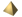
\includegraphics[width=0.7cm]{pyramid} This is a raster
%%that has pyramids built for it to improve rendering efficiency (see
%%Section \ref{raster_pyramids}).\\
%%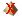
\includegraphics[width=0.7cm]{no_pyramid} This is a
%%raster that has no pyramid layers (see Section \ref{raster_pyramids}).\\
%%
\includegraphics[width=0.7cm]{inoverview} This layer is
%%shown in the overview map area as well as in the main map window.\\
%%
\includegraphics[width=0.7cm]{editable} This is a vector
%%layer that is currently enabled for editing.\\
%
%\subsubsection{Map View}\label{label_mapview}
%\index{map!view}

%%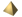
\includegraphics[width=0.7cm]{pyramid} Ceci est un raster doté de pyramides qui améliorent son affichage (voir Section \ref{raster_pyramids}).\\
%% 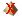
\includegraphics[width=0.7cm]{no_pyramid} Ce raster ne dispose pas de pyramides (see Section \ref{raster_pyramids}).\\
%% 
\includegraphics[width=0.7cm]{inoverview} Cette couche est affichée dans la zone d'aperçu ainsi que la fenêtre principale.\\
%% 
\includegraphics[width=0.7cm]{editable} Cette couche vecteur est activée pour l'édition.\\

\subsubsection{Vue de la carte}\label{label_mapview}
\index{map!view}

%This is the 'business end' of QGIS - maps are displayed in this area! The
%map displayed in this window will depend on the vector and raster layers you
%have chosen to load (see sections that follow for more information on how to
%load layers). The map view can be panned (shifting the focus of the map display
%to another region) and zoomed in and out. Various other operations can be
%performed on the map as described in the toolbar description above.  The map
%view and the legend are tightly bound to each other - the maps in view reflect
%changes you make in the legend area.  

C'est la partie centrale de QGIS — les cartes sont affichées dans cette partie ! Celle qui s'affiche dépend des couches raster et vecteurs que vous avez choisi de charger (lire les sections suivantes pour savoir comment charger une couche). La vue de la carte peut être modifiée en portant le focus sur une autre région, ou en zoomant en avant ou en arrière. Plusieurs opérations peuvent être effectuées sur la carte comme il est expliqué dans les descriptions des barres d'outils. La vue de la carte et la légende sont étroitement liées — la carte reflète les changements que vous opérez dans la légende.

%\begin{Tip}\caption{\textsc{Zooming the Map with the Mouse
%Wheel}}\index{zoom!mouse wheel}
%\qgistip{You can use the mouse wheel to zoom in and out on the map. Place
%the mouse cursor inside the map area and roll the wheel forward (away from you) to
%zoom in and backwards (towards you) to zoom out. The mouse cursor position is the 
%center where the zoom occurs. You can customize the behavior of the mouse
%wheel zoom using the \tab{Map tools} tab under the \mainmenuopt{Settings} >\dropmenuopt{Options} menu.  }
%\end{Tip}

\begin{Astuce}\caption{\textsc{Zoomer la carte avec la molette de la souris}\index{zoom!mouse wheel}}
\qgistip{Vouspouvez utiliser la molette de la souris pour changer le niveau de zoom de la carte. Placez votre curseur dans la zone d'affichage de la carte et faites rouler la molette vers l'avant pour agrandir et faites là rouler vers vous pour zoomer en arrière. La position du curseur est le centre sur lequel va s'opérer le zoom. Vous pouvez modifier le comportement du zoom de la souris en utilisant l'onglet \tab{Outils cartographiques} dans le menu \mainmenuopt{Paramètres} >\dropmenuopt{Options}.}
\end{Astuce}

%\begin{Tip}\caption{\textsc{Panning the Map with the Arrow Keys and Space Bar}}\index{pan!arrow keys}
%\qgistip{You can use the arrow keys to pan in the map. Place the mouse cursor 
%inside the map area and click on the right arrow key to pan East, left arrow 
%key to pan West, up arrow key to pan North and down arrow key to pan South. 
%You can also pan the map using the space bar: just move the mouse while
%holding down space bar.
%}
%\end{Tip}

\begin{Astuce}\caption{\textsc{Déplacer la carte avec les flèches et la barre espace}}\index{pan!arrow keys}
\qgistip{Vous pouvez utiliser les flèches du clavier pour se déplacer sur la carte? Placez le curseur sur la carte et appuyez sur la flèche droite pour vous diriger vers l'Est, la flèche gauche pour aller vers l'Ouest, la flèche supérieure pour le Nord et la flèche inférieure pour le Sud. Vous pouvez aussi déplacer la carte en gardant la touche espace appuyée et en bougeant la souris.
}
\end{Astuce}

%\subsubsection{Map Overview}\label{label_mapoverview}
%\index{map!overview}
%
%The map overview area provides a full extent view of layers added to it.
%Within the view is a rectangle showing the current map extent. This allows
%you to quickly determine which area of the map you are currently viewing. Note
%that labels are not rendered to the map overview even if the layers in the
%map overview have been set up for labeling. 
%You can add a single layer to the overview by right-clicking on it in the legend 
%and select \checkbox{Show in overview}. You can also add layers to, or remove 
%all layers from the overview using the Overview tools on the toolbar.
%
%If you click and drag the red rectangle in the overview that shows your 
%current extent, the main map view will update accordingly.

\subsubsection{Aperçu de la carte}\label{label_mapoverview}
\index{map!overview}

La zone d'aperçu de la carte permet d'avoir une vue totale de l'emprise des couches ajoutées au projet. Au sein de cette fenêtre se situe un rectangle qui représente l'étendue de la carte, cela permet de savoir quelle région de la carte vous êtes en train de visualiser. Les étiquettes ne sont pas affichées dans l'aperçu même si les couches visibles ont l'affichage de leurs étiquettes activées.
Vous pouvez rajoutez une couche dans l'aperçu en faisant un clic-droit dessus dans la légende ou en sélectionnant \checkbox{Montrer dans l'aperçu}. Vous pouvez aussi rajouter des couches ou en ôter de l'aperçu en utilisant les outils d'aperçu dans la barre d'outils.

Si vous cliquez et déplacez le rectangle rouge qui montre votre emprise actuelle, la vue principale se mettra en conséquence.

%\subsubsection{Status Bar}\label{label_statusbar}
%
%The status bar shows you your current position in map coordinates (e.g.
%meters or decimal degrees) as the mouse pointer is moved across the map view.
%To the left of the coordinate display in the status bar is a small button that 
%will toggle between showing coordinate position or the view extents of the 
%map view as you pan and zoom in and out. 
%
%A progress bar in the status bar shows progress of rendering
%as each layer is drawn to the map view. In some cases, such as the gathering
%of statistics in raster layers, the progress bar will be used to show the
%status of lengthy operations. 
%
%If a new plugin or a plugin update is available, you will see a message in the 
%status bar. On the right side of the status bar is a small
%checkbox which can be used to temporarily prevent layers being rendered to the
%map view (see Section \ref{subsec:redraw_events} below). At the far right of
%the status bar is a projector icon. Clicking on this opens the projection
%properties for the current project.

\subsubsection{Barre de statuts}\label{label_statusbar}

La barre de statuts montre votre position dans les coordonnées de la carte (p. ex. mètres ou degrés décimaux) lorsque vous déplacez votre curseur. À gauche de l'affichage des coordonnées se trouve un petit bouton qui bascule entre les coordonnées de la position ou l'étendue de la zone que vous visualisez.

Une barre de progression dans la barre de statuts vous montre le cheminement du rendu au fur et à mesure qu'une couche est dessinée sur l'écran. Dans certains cas, tel que lors de l'établissement de statistiques d'une couche raster, la barre indique le statut des opérations qui prennent du temps.

Si une nouvelle extension ou une mise à jour est disponible, vous verrez un message dans la barre de statut. Sur la droite, une boîte à cocher peut être utilisée pour bloquer le rendu des couches sur la carte (voir Section \ref{subsec:redraw_events}). A l'extrémité se situe l'icône de projection,  un clic dessus ouvrira la fenêtre de propriétés de projection pour le projet en cours.

%\begin{Tip}\caption{\textsc{Calculating the correct Scale of your Map Canvas}}\index{scale!calculate}
%\qgistip{When you start QGIS, degrees is the default unit, and it tells QGIS 
%that any coordinate in your layer is in degrees. To get correct scale values, 
%you can either change this to meter manually in the \tab{General} tab under 
%\mainmenuopt{Settings} >\dropmenuopt{Project Properties} or you can select a project 
%Coordinate Reference System (CRS) clicking on the \toolbtntwo{mIconProjectionEnabled}{projector} 
%icon in the lower right-hand corner of the statusbar. In the last case, the 
%units are set to what the project projection specifies, e.g. '+units=m'.
%}
%\end{Tip}

\begin{Astuce}\caption{\textsc{Calculer l'échelle correcte de la vue de la carte}}\index{scale!calculate}
\qgistip{Quand vous démarrez QGIS, les degrés sont l'unité par défaut et indique à QGIS que toutes les coordonnées de votre couche sont en degrés. Pour avoir les valeurs correctes de l'échelle, vous pouvez soit passer en mètre manuellement avec l \tab{General} sous le menu \mainmenuopt{Préférences} >\dropmenuopt{Propriétés du projet} ou vous pouvez sélectionner un système de projection de référence en cliquant sur \toolbtntwo{mIconProjectionEnabled}{projector}. Dans ce dernier cas, les unités sont automatiquement choisies selon les spécifications de la projection, p. ex. '+units=m'.
}
\end{Astuce}

%\subsection{Rendering}\label{subsec:redraw_events}\index{rendering}
%
%By default, QGIS renders all visible layers whenever the map canvas must be
%refreshed. The events that trigger a refresh of the map canvas include:
%
%\begin{itemize}
%\item Adding a layer
%\item Panning or zooming
%\item Resizing the QGIS window
%\item Changing the visibility of a layer or layers
%\end{itemize}
%
%QGIS allows you to control the rendering process in a number of ways.

\subsection{Rendu}\label{subsec:redraw_events}\index{rendering}

Par défaut, QGIS effectue le rendu de toutes les couches visibles à chaque fois que l'affichage de la carte a besoin d'être mise à jour. Les événements qui déclenchent ce rafraîchissement incluent :

\begin{itemize}
\item L'ajout d'une couche
\item Un déplacement ou un zoom
\item Un redimensionnement de la fenêtre de QGIS
\item Un changement de la visibilité d'une couche
\end{itemize}

%\subsubsection{Scale Dependent Rendering}\index{rendering!scale dependent}
%\label{label_scaledepend}
%
%Scale dependent rendering allows you to specify the minimum and maximum
%scales at which a layer will be visible.  To set scale dependency rendering,
%open the \dialog{Properties} dialog by double-clicking on the layer in the 
%legend. On the \tab{General} tab, set the minimum and maximum scale values and then
%click on the \checkbox{Scale dependent visibility} checkbox.
%
%You can determine the scale values by first zooming to the level you want
%to use and noting the scale value in the QGIS status bar.\index{scale}
%
%\subsubsection{Controlling Map Rendering}\label{label_controlmap}
%
%Map rendering can be controlled in the following ways:

\subsubsection{Rendu dépendant de l'échelle}\index{rendering!scale dependent}
\label{label_scaledepend}

Le rendu dépendant de l'échelle permet de spécifier l'échelle minimale et maximale à laquelle la couche doit être visible. Pour définir une échelle de rendu, ouvrez la fenêtre de \dialog{Propriétées} en double-cliquant sur une couche dans la légende et dans l'onglet \tab{Général}, saisissez les valeurs voulues et cocher la case \checkbox{Utiliser le rendu dépendant de la mise à l'échelle}.

Vous pouvez déterminer les valeurs d'échelle en zoomant au niveau que vous voulez utiliser et en notant les valeurs de la barre d'état.\index{scale}

\subsubsection{Contrôler le rendu}\label{label_controlmap}

Le rendu de la carte peut être contrôlé de différentes manières :

%\minisec{a) Suspending Rendering}\index{rendering!suspending}
%\label{label_suspendrender}
%
%To suspend rendering, click the \checkbox{Render} checkbox in the lower right
%corner of the statusbar. When the \checkbox{Render} box is not checked, QGIS
%does not redraw the canvas in response to any of the events described in
%Section \ref{subsec:redraw_events}. Examples of when you might want to suspend
%rendering include:
%
%\begin{itemize}
%\item Add many layers and symbolize them prior to drawing
%\item Add one or more large layers and set scale dependency before drawing
%\item Add one or more large layers and zoom to a specific view before drawing
%\item Any combination of the above
%\end{itemize}
%
%Checking the \checkbox{Render} box enables rendering and causes and immediate
%refresh of the map canvas.

\minisec{a) Suspendre le rendu}\index{rendering!suspending}
\label{label_suspendrender}

Pour suspendre le rendu, cliquez sur la case \checkbox{Render}dans le coin inférieur droit de la barre de statut. Quand cette case n'est pas coché, QGIS ne redessine pas la carte en réponse aux événements décrits dans la section \ref{subsec:redraw_events}. Voici quelques cas pour lequel vous pourriez vouloir le faire :

\begin{itemize}
\item Ajouter beaucoup de couches et les symboliser avant d'effectuer un rendu potentiellement long
\item Ajouter une ou plusieurs couches et définir une échelle
\item Ajouter une ou plusieurs couches et et zoomer sur un endroit spécifique
\item N'importe quelle combinaison des éléments précédents
\end{itemize}

Cocher la case \checkbox{Rendu} activera de nouveau le rendu et provoquera un rafraîchissement immédiat de la vue active.

%\minisec{b) Setting Layer Add Option}\label{label_settinglayer}
%\index{rendering!options}\index{layers!initial visibility}
%
%You can set an option to always load new layers without drawing them. This
%means the layer will be added to the map, but its visibility checkbox in the
%legend will be unchecked by default. To set this option, choose
%menu option \mainmenuopt{Settings} > \dropmenuopt{Options} and click on the
%\tab{Rendering} tab. Uncheck the \checkbox{By default new layers added to the map 
%should be
%displayed} checkbox. Any layer added to the map will be off (invisible) by
%default.

\minisec{b) Définir les options d'ajout de couche}\label{label_settinglayer}
\index{rendering!options}\index{layers!initial visibility}

Il est possible de définir une option qui chargera toutes les nouvelles couches sans les dessiner, elles seront ajoutées à la carte, mais la case de visibilité sera décochée par défaut. Pour définir cette option, sélectionnez l'option \mainmenuopt{Préférences} > \dropmenuopt{Options} et cliquez sur l'onglet \tab{Rendu}. Décochez la case \checkbox{par défaut les couches supplémentaires sont affichées}. Les nouvelles couches ajoutées à la carte seront invisibles par défaut.

%%\minisec{Stopping Rendering}\index{rendering!halting}
%%\label{label_stoprender}
%%
%%To stop the map drawing, press the ESC key. This will halt the refresh of
%%the map canvas and leave the map partially drawn. It may take a bit of time
%%between pressing ESC and the time the map drawing is halted.
%%
%%\textbf{NOTE}: It is currently not possible to stop rendering - this was disabled 
%%in qt4 port because of User Interface (UI) problems and crashes.

\minisec{Arrêter le rendu}\index{rendering!halting}
\label{label_stoprender}

Pour arrêter le rendu de la carte, appuyez sur la touche ESC. Ceci stoppera le rafraîchissement de la vue de la carte et laissera la carte partiellement dessinée. Il est possible qu'il y ait un délai entre le moment où la touche est pressée et le temps que le rendu de la carte soit arrêté.

\textbf{NOTE}: Il n'est pas actuellement possible d'arrêter le rendu de cette manière — ça été désactivé avec le port qt4 du fait d'instabilités.

%\minisec{c) Updating the Map Display During Rendering}
%\label{label_updatemap}\index{rendering!update during drawing}
%
%You can set an option to update the map display as features are drawn. By
%default, QGIS does not display any features for a layer until the entire
%layer has been rendered. To update the display as features are read from the
%datastore, choose menu option \mainmenuopt{Settings} > \dropmenuopt{Options}
%click on the \tab{Rendering} tab. Set the feature count to an
%appropriate value to update the display during rendering. Setting a value of 0
%disables update during drawing (this is the default). Setting a value too low
%will result in poor performance as the map canvas is continually updated
%during the reading of the features. A suggested value to start with is 500. 

\minisec{c) Mettre la jour l'affichage de la carte pendant le rendu}
\label{label_updatemap}\index{rendering!update during drawing}

Vous pouvez définir une option pour mettre à jour l'affichage de la carte quand des entités sont dessinées. Par défaut, QGIS n'affiche pas les entités d'une couche tant que la couche entière n'a pas été rendue. Pour mettre à jour l'affichage à mesure que les entités sont lues dans la table attributaire, sélectionnez le menu \mainmenuopt{Settings} > \dropmenuopt{Options} puis l'onglet \tab{Rendu}. Mettez comme valeur le nombre d'entités à mettre à jour durant le rendu. Si elle est égale à 0 cela désactive la mise à jour durant le dessin (c'est la valeur par défaut). Une valeur trop basse risque d'impacter les performances, car la vue de la carte sera constamment mise à jour durant la lecture des entités. Il est suggéré de commencer à 500.

%\minisec{d) Influence Rendering Quality}
%\label{label_renderquality}\index{rendering!quality}
%
%To influence the rendering quality of the map you have 3 options. Choose menu 
%option \mainmenuopt{Settings} > \dropmenuopt{Options} click on the 
%\tab{Rendering} tab and select or deselect following checkboxes.
%
%\begin{itemize}
%\item \checkbox{Make lines appear less jagged at the expense of some drawing performance}
%\item \checkbox{Fix problems with incorrectly filled polygons}
%\item \checkbox{Continuously redraw the map when dragging the legend/map divider}
%\end{itemize}

\minisec{d) Influencer la qualité du rendu}
\label{label_renderquality}\index{rendering!quality}

Pour influencer la qualité du rendu de la carte vous avez trois possibilités. Dans le menu \mainmenuopt{Préférences} > \dropmenuopt{Options} puis l'onglet \tab{Rendu} et sélectionnez/désélectionnez les cases suivantes :

\begin{itemize}
\item \checkbox{Les lignes semblent moins déchiquetées aux dépends d'une certaine vitesse d'exécution}
\item \checkbox{Corriger les polygones remplis de manière erronée}
\item \checkbox{Rafraîchir en permanence lors du déplacement de la table des matières/carte}
\end{itemize}

%\subsection{Measuring}\label{sec:measure}\index{measure}
%
%Measuring works within projected coordinate systems only (e.g., UTM). If 
%the loaded map is defined with a geographic coordinate system
%(latitude/longitude), the results from line or area measurements will be 
%incorrect. To fix this you need to set an appropriate map coordinate system 
%(See Section~\ref{label_projections}).

\subsection{Mesurer}\label{sec:measure}\index{measure}

Les mesures fonctionnent uniquement au sein des systèmes de coordonnées projetées (exemple : UTM, Lambert 93). SI la couche active est définie par système géographique de coordonnée (latitude/longitude), les résultats d'une mesure de ligne ou d'aires seront incorrects. Pour y remédier, vous devez mettre un système de coordonnées approprié (voir Section~\ref{label_projections}).

%\subsubsection{Measure length and areas}\index{measure:line length}\index{measure:areas}
%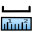
\includegraphics[width=0.7cm]{mActionMeasure} 
%QGIS is also able to measure real distances between given 
%points according to a defined ellipsoid. To configure this, choose menu option 
%\mainmenuopt{Settings} > \dropmenuopt{Options}, 
%click on the \tab{Map tools} tab and choose the appropriate ellipsoid. The tool then allows you to 
%click points on the map. Each segment-length shows up in the measure-window and additionally the total 
%length is printed. To stop measuring click your right mouse button. \\
%
\includegraphics[width=0.7cm]{mActionMeasureArea} Areas can also be measured. 
%The window shows the accumulated area-size in the measure window 

\subsubsection{Mesurer une longueur et une aire}\index{measure:line length}\index{measure:areas}
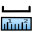
\includegraphics[width=0.7cm]{mActionMeasure} 
QGIS peut mesurer des distances réelles entre plusieurs points selon un ellipsoïd défini. Pour le configurer, allez dans le menu \mainmenuopt{Préférences} > \dropmenuopt{Options}puis dans l'onglet \tab{Outils cartographiques} et choisissez l'ellipsoïde approprié. Cet outil permet de placer des points sur la carte. Chaque longueur de segment s'affiche dans la fenêtre de mesure avec la longueur additionnée totale. Pour stopper les mesures, faites un clic droit. \\

\includegraphics[width=0.7cm]{mActionMeasureArea} Les aires peuvent aussi être mesurées.

\begin{figure}[h]
\caption{Outils de mesure \nixcaption} \label{fig:measure}
\centering
  \subfigure[Mesure de lignes] {\label{subfig:measure_line}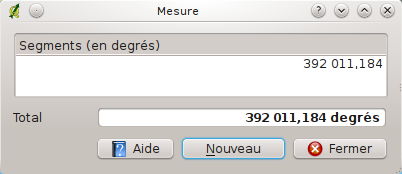
\includegraphics[clip=true, width=0.3\textwidth]{measure_line}}\goodgap
  \subfigure[Mesure d'aires]{\label{subfig:measure_area}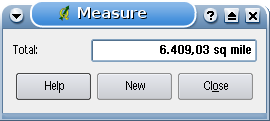
\includegraphics[clip=true, width=0.3\textwidth]{measure_area}}
\end{figure}

%\subsection{Projects}\label{sec:projects}\index{projects}
%
%The state of your QGIS session is considered a Project.  QGIS
%works on one project at a time.  Settings are either considered
%as being per-project, or as a default for new projects (see
%Section \ref{subsec:gui_options}). QGIS can save the state of your 
%workspace into a project file using the menu options 
%\mainmenuopt{File} > \dropmenuopttwo{mActionFileSave}{Save Project}
%or \mainmenuopt{File} > \dropmenuopttwo{mActionFileSaveAs}{Save Project As}.
%
%Load saved projects into a QGIS session using 
%\mainmenuopt{File} > \dropmenuopttwo{mActionFileOpen}{Open Project}
%or \mainmenuopt{File} > \dropmenuopt{Open Recent Project}.
%If you wish to clear your session and start fresh, choose
%\mainmenuopt{File} > \dropmenuopttwo{mActionFileNew}{New Project}.
%Either of these menu options will prompt you to save the existing project
%if changes have been made since it was opened or last saved.
%
%The kinds of information saved in a project file include:

\subsection{les projets}\label{sec:projects}\index{projets}

L'état de votre session de QGIS est considéré comme étant un projet. QGIS ne peut travailler que sur un projet à la fois. Les propriétés sont considérées comme étant assignées à un projet ou comme étant par défaut pour les nouveaux projets ( voir Section \ref{subsec:gui_options}). QGIS peut enregistrer l'état de votre travail dans un fichier de projet en utilisant le menu the state of your 
workspace into a project file using the menu options 
\mainmenuopt{Fichier} > \dropmenuopttwo{mActionFileSave}{Sauvegarder le projet}
or \mainmenuopt{File} > \dropmenuopttwo{mActionFileSaveAs}{Sauvegarder le projet sous...}.

Pour charger un projet dans une session QGIS, aller dans \mainmenuopt{Fichier} > \dropmenuopttwo{mActionFileOpen}{Ouvrir un Projet} ou \mainmenuopt{Fichier} > \dropmenuopt{Ouvrir un projet récent}. Si vous souhaitez revenir à une session vierge, aller sur \mainmenuopt{Fichier} > \dropmenuopttwo{mActionFileNew}{Nouveau Projet}.
Chacune de ces options vous demandera si vous désirez enregistrer le projet si des changements ont été effectués depuis son ouverture ou sa dernière sauvegarde.

Les type d'informations enregistrées dans un projet sont :

\begin{itemize}
\item Les couches ajoutées
\item Les propriétés des couches ainsi que de symbologie
\item La projection de la carte
\item L'étendue de la dernière zone de visualisation
\end{itemize}
%
%The project file is saved in XML format, so it is possible to edit
%the file outside QGIS if you know what you are doing. The file format 
%was updated several times compared to earlier QGIS versions. Project files 
%from older QGIS versions may not work properly anymore. To be made aware of this, 
%in the \tab{General} tab under \mainmenuopt{Settings} > \dropmenuopt{Options} 
%you can select \checkbox{Warn when opening a project file saved with an older 
%version of QGIS}.


Le fichier de projet est enregistré au format XML, il est donc possible de l'éditer en dehors de QGIS si vous savez ce que vous faites. Le format a été modifié à plusieurs reprises depuis les versions antérieures de QGIS, les fichiers enregistrés sous ces dernières peuvent ne plus fonctionner correctement. Pour être averti dans genre de cas, allez dans l'onglet \tab{General} du menu \mainmenuopt{Préférences} > \dropmenuopt{Options} et sélectionnez \checkbox{M'avertir lors de l'ouverture d'un fichier projet sauvegardé avec une version précédente de QGIS}.

%\subsection{Output}\label{sec:output}\index{output!save as image!print composer!quick print}
%There are several ways to generate output from your QGIS session.
%We have discussed one already in Section \ref{sec:projects}: saving as a project file. 
%Here is a sampling of other ways to produce output files:
%\begin{itemize}
%\item Menu option \dropmenuopttwo{mActionSaveMapAsImage}{Save as Image} opens a
%file dialog where you select the name, path and type of image (PNG or JPG format).
%\item Menu option \dropmenuopttwo{mActionFilePrint}{Print Composer} opens a dialog 
%where you can layout and print the current map canvas (see Section~\ref{label_printcomposer}).
%\end{itemize}

\subsection{Sauvegarder l'affichage}\label{sec:output}\index{output!save as image!print composer!quick print}
Il y a plusieurs façons d'enregistrer un fichier depuis votre session. Nous en avons déjà vu une dans la section \ref{sec:projects} : sauvegarder dans un fichier de projet.
Voici d'autres manières de procéder à l'enregistrement de fichiers :
\begin{itemize}
\item Menu option \dropmenuopttwo{mActionSaveMapAsImage}{Sauvagarder comme une Image} ouvre une fenêtre de dialogue où vous devez saisir le nom, le chemin et le types d'images (PNG ou JPEG).
\item Menu option \dropmenuopttwo{mActionFilePrint}{Paramètrage de l'impression} ouvre une fenêtre de dialogue où vous pouvez faire une mise en page et imprimer la vue active de la carte (voir Section~\ref{label_printcomposer}).
\end{itemize}

%\subsection{GUI Options}
%\label{subsec:gui_options}
%
\includegraphics[width=0.7cm,clip=true]{mActionOptions} 
%Some basic options for QGIS
%can be selected using the \dialog{Options} dialog. Select the 
%menu option \mainmenuopt{Settings} >
% \dropmenuopttwo{mActionOptions}{Options}. The tabs where you can 
%optmize your options are:

\subsection{Options d'affichage}
\label{subsec:gui_options}

\includegraphics[width=0.7cm,clip=true]{mActionOptions} 
Quelques options basiques peuvent être sélectionnés en allant dans le menu \mainmenuopt{Préférences} >
\dropmenuopttwo{mActionOptions}{Options}. Les onglets dans lesquels vous pouvez configurer les options sont :

%\minisec{General Tab}
%
%\begin{itemize}
%\item \checkbox{Ask to save project changes when required}
%\item \checkbox{Warn when opening a project file saved with an older version of QGIS}
%\item \checkbox{Change Selection and backgroud Color}
%\item Change the icon theme (choose between default, classic, gis and nkids)
%\item \checkbox{Capitalise layer names in legend}
%\item \checkbox{Display classification attribute names in legend}
%\item \checkbox{Hide splash screen at startup}
%\item \checkbox{Open attribute table in a dock window}
%\item Define attribute table behavior (choose between show all features, show 
%selected features and show features in current canvas)
%\end{itemize}

\minisec{onglet Général}

\begin{itemize}
\item \checkbox{Demander à sauvegarder les changements apportés au projet si requis}
\item \checkbox{M'avertir lors de l'ouverture d'un fichier projet sauvegardé avec une version précédente de QGIS}
\item \checkbox{Changer la couleur de la sélection du fond d'écran}
\item Changer le thème des icônes
\item \checkbox{Mettre les noms de couche en majuscule dans la légende}
\item \checkbox{Afficher les noms des attributs de classifications dans la légende}
\item \checkbox{Cacher l'écran de démarrage}
\item \checkbox{Ouvrir la table d'attributs dans une fenêtre mobile}
\item Définir le comportement de la table d'attributs (choisir entre montrer toutes les entités, celles sélectionnées et celles présentes dans la vue active)
\end{itemize}

%\minisec{Rendering Tab}
%
%\begin{itemize}
%\item \checkbox{By deafult new layers added to the map should be displayed}
%\item Define number of features to draw before updating the display.
%\item \checkbox{Make lines appear less jagged at the expense of some drawing performance}
%\item \checkbox{Fix problems with incorrectly filled polygons}
%\item \checkbox{Continously redraw when dragging the legend/map divider} 
%\end{itemize}

\minisec{Onglet de Rendu}

\begin{itemize}
\item \checkbox{Par défaut les couches supplémentaires sont affichées}
\item Définir le nombre d'entités à dessiner avant d'actualiser l'affichage.
\item \checkbox{Les lignes semblent moins déchiquetées aux dépens d'une certaine vitesse d'exécution}
\item \checkbox{Corriger les polygones remplis de manière erronée}
\item \checkbox{Rafraîchir en permanence la table des matières/carte lors du déplacement} 
\end{itemize}

%\minisec{Map tools Tab}
%
%\begin{itemize}
%\item Define Search Radius as a percentage of the map width
%\item Define Ellipsoid for distance calculations
%\item Define Rubberband Color for Measure Tools
%\item Define Mouse wheel action (Zoom, Zoom and récenter, Zoom to mouse cursor, Nothing)
%\item Define Zoom factor for wheel mouse
%\end{itemize}

\minisec{Onglet des Outils Cartographiques}

\begin{itemize}
\item Spécifier le rayon de recherche comme pourcentage de la largeur de la carte)
\item Définir l'ellipsoïde pour des calculs de distance
\item Définir la couleur de l'étirement pour les outils de mesure
\item Définir l'action de la molette de la souris (Zoomer, Zoomer et récentrer, Zoomer sur le curseur de la souris, Rien)
\item Définir le facteur de zoom
\end{itemize}

%\minisec{Digitizing Tab}
%
%\begin{itemize}
%\item Define Rubberband Color and line width for Digitizing
%\item Define default snap mode (to vertex, to segment, to vertex and segment)
%\item Define default snapping tolerance in layer units
%\item Define search radius for vertex edits in layer units
%\item Define vertex marker style (Cross or semi transparent circle)
%\end{itemize}

\minisec{Onglet de Nuémrisation}

\begin{itemize}
\item Définir la couleur et la largeur de la ligne d'étirement
\item Définir le mode d'accrochage par défaut (à un vertex, un segment, aux vertex et segments)
\item Définir la tolérance d'accrochage par défaut (en unités de la couche) 
\item Définir le rayon de recherche pour l'édition des sommets (en unités de la couche) 
\item Définir les marqueurs de sommet (croix ou cercle semi-transparent)
\end{itemize}

%\minisec{CRS Tab}
%
%\begin{itemize}
%\item \checkbox{Prompt for Coordinate Reference System (CRS)}
%\item \checkbox{Project wide default Coordinate Reference System (CRS) will be used}
%\item \checkbox{Global default Coordinate Reference System (CRS) displayed below will be used}
%\item Select global default Coordinate Reference System (CRS)

\minisec{Onglet de SCR}

\begin{itemize}
\item \checkbox{Demander pour le Système de Coordonnées de Référence (SCR)}
\item \checkbox{La projection globale par défaut du projet qui sera employée. }
\item \checkbox{La projection par défaut ci-dessous sera employée. }
\item Sélectionner le Système de Coordonnées de Référence (SCR) par défaut
\end{itemize}

%\minisec{Locale Tab}
%
%\begin{itemize}
%\item \checkbox{Overwrite system locale and use defined locale instead}
%\item Information about active system locale
%\end{itemize}

\minisec{Onglet de Paramètres du lieu}

\begin{itemize}
\item \checkbox{Forcer la nationalité du système}
\item Paramètres de lieu sur votre système 
\end{itemize}

%\minisec{Proxy Tab}
%
%\begin{itemize}
%\item \checkbox{Use proxy for web access} and define host, port, user, and password.
%\end{itemize}
%
%You can modify the options according to your needs. Some of the changes may 
%require a restart of QGIS before they will be effective.
%
%\begin{itemize}
%\item \nix{settings are saved in a texfile: \$HOME/.config/QuantumGIS/qgis.conf}
%\item \osx{you can find your settings in: \$HOME/Library/Preferences/org.qgis.qgis.plist}
%\item \win{settings are stored in the registry under:}
%\begin{verbatim}
%\\HKEY\CURRENT\USER\Software\QuantumGIS\qgis
%\end{verbatim}
%\end{itemize}

\minisec{Onglet Proxy}

\begin{itemize}
\item \checkbox{Utiliser un proxy pour l'accés internet} et définition de l'hôte, du port, de l'utilisateur et du mot de passe.
\end{itemize}

Vous pouvez modifier ces options selon vos besoins, certains de ces changements nécessiteront un redémarrage avant d'être effectifs.

\begin{itemize}
\item \nix{les paramètres sont enregistrés dans un fichier texte: \$HOME/.config/QuantumGIS/qgis.conf}
\item \osx{les paramètres sont enregistrés dans: \$HOME/Library/Preferences/org.qgis.qgis.plist}
\item \win{les paramètres sont enregistrés dans le registre sous:}
\begin{verbatim}
\\HKEY\CURRENT\USER\Software\QuantumGIS\qgis
\end{verbatim}
\end{itemize}

%\subsection{Spatial Bookmarks}\label{sec:bookmarks}
%\index{bookmarks}
%\index{spatial bookmarks|\see{bookmarks}}
%
%Spatial Bookmarks allow you to ``bookmark'' a geographic location and return to it later.
%
%\subsubsection{Creating a Bookmark}
%To create a bookmark:
%\begin{enumerate}
%\item Zoom or pan to the area of interest.
%\item Select the menu option \mainmenuopt{View} > \dropmenuopt{New Bookmark} or press \keystroke{Ctrl-B}.
%\item Enter a descriptive name for the bookmark (up to 255 characters).
%\item Click \button{OK} to add the bookmark or \button{Cancel} to exit without adding the bookmark.
%\end{enumerate}
%
%Note that you can have multiple bookmarks with the same name.

\subsection{Signets spatiaux}\label{sec:bookmarks}
\index{bookmarks}
\index{spatial bookmarks|\see{bookmarks}}

Les signets spatiaux vous permettent de marquer une zone de la carte pour y retourner plus tard.

\subsubsection{Créer un signet}
Pour créer un signet :
\begin{enumerate}
\item Déplacez-vous sur la zone concernée
\item Sélectionnez le menu \mainmenuopt{Vue} > \dropmenuopt{Nouveau signet} ou appuyez sur la touche \keystroke{Ctrl-B}.
\item Entrez un nom pour décrire le signet (jusqu'à 255 caractères).
\item Cliquez sur \button{OK} pour ajouter le signet ou sur \button{Annuler} pour sortir de la fenêtre sans l'enregistrer.
\end{enumerate}

Vous pouvez avoir plusieurs signets portant le même nom.

%\subsubsection{Working with Bookmarks}
%To use or manage bookmarks, select the menu 
%option \mainmenuopt{View} > \dropmenuopt{Show Bookmarks}.
%The \dialog{Geospatial Bookmarks} dialog allows you to zoom to or delete a bookmark.
%You can not edit the bookmark name or coordinates.
%
%\subsubsection{Zooming to a Bookmark}
%From the \dialog{Geospatial Bookmarks} dialog, select the desired bookmark by clicking on it, 
%then click \button{Zoom To}.
%You can also zoom to a bookmark by double-clicking on it.

\subsubsection{Travailler avec les signets}
Pour utiliser ou gérer les signets allez dans le menu \mainmenuopt{Vue} > \dropmenuopt{Montrer les signets}.
Le dialogue \dialog{Signets géospatiaux} vous permet de zoomer ou d'effacer un signet.
Vous ne pouvez pas modifier le nom d'un signet ou ses coordonnées.

\subsubsection{Zoomer sur un signet}
Depuis la fenêtre \dialog{Signets géospatiaux}, sélectionner le signet voulu en cliquant dessus puis sur le bouton \button{Zoomer sur}. Vous pouvez aussi zoomer en opérant un double-clic.

%\subsubsection{Deleting a Bookmark}
%To delete a bookmark from the \dialog{Geospatial Bookmarks} dialog, click on it then click
% \button{Delete}.
%Confirm your choice by clicking \button{Yes} or cancel the delete by clicking \button{No}.

\subsubsection{Effacer un signet}
Pour effacer un signet depuis la fenêtre \dialog{Signets géospatiaux}, cliquez dessus puis sur le bouton \button{Effacer}.
Confirmez votre choix en cliquant sur \button{Oui} ou annuler en cliquant sur \button{Non}.
